\documentclass[12pt,a4paper]{article}
\usepackage[utf8]{inputenc}
\usepackage{amsmath}
\usepackage{amsfonts}
\usepackage{amssymb}
\usepackage{listings}
\usepackage{url}
\usepackage[bulgarian]{babel}
\usepackage{listings}
\usepackage{enumerate}
\usepackage{hyperref}
\usepackage{relsize}
\usepackage{graphicx}


\lstset{breaklines=true} 


\author{\textit{email: kalin@fmi.uni-sofia.bg}}
\title{\textsc{Задачи за задължителна самоподготовка} \\
по \\
Структури от данни и програмиране\\
\textit{Двоични дървета}}



\begin{document}
\maketitle


\begin{enumerate}


	\item Да се деифнира метод \texttt{count} на клас \texttt{BTree}, който намира броя на елементите на дървото.

	\item Да се деифнира метод \texttt{countEvens} на клас \texttt{BTree}, който намира броя на елементите на дърво от числа, които са четни.


	\item Да се дефинира метод \texttt{int BTree<T>::searchCount (bool (*pred)(const T\&))} към клас \texttt{BTree}, който намира броя на елементите на дървото, които удовлетворяват предиката \texttt{pred}.

	Да се приложи \texttt{searchCount} за решаване на горните две задачи.


	\item Да се дефинира метод \texttt{bool BTree<T>::height ()}, намиращ височината на дърво.

	\begin{flushleft}
	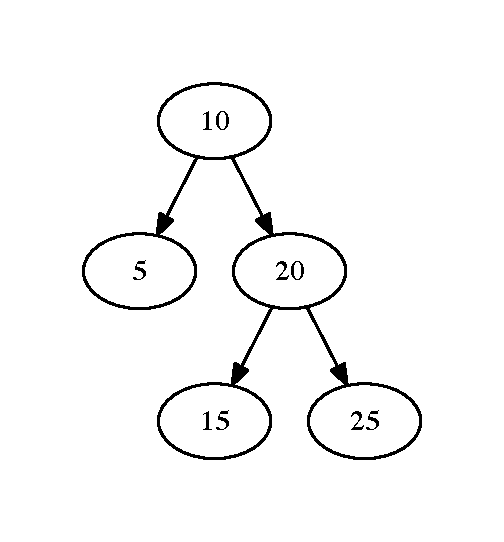
\includegraphics[width=4cm]{images/tree1}

	\relscale{0.8}
	Фигура 1. Двоично наредено дърво
	\end{flushleft}


	\textit{Височина на дърво наричаме дължината (в брой върхове) на най-дългия път от корена до кое да е листо на дървото.}

	\textit{Пример. Височината на дървото на фигура 1 е \textbf{3}.}


	\item Да се деифнира метод \texttt{countLeaves} на клас \texttt{BTree}, който намира броя на листата в дървото.

	\item Да се деифнира метод \texttt{maxLeaf} на клас \texttt{BTree}, който намира най-голямото по стойност листо на непразно дърво. Да се приеме, че за типа \texttt{T} на шаблона \texttt{BTree} е дефиниран операторът \texttt{<}.


	\item Нека е дадено дървото \texttt{t} и низът \texttt{s}, съставен само от символите `L' и `R' ($s \in \{L,R\}^*$). Нека дефинираме ``съответен елемент'' на низа \texttt{s} в дървото \texttt{t} по следния начин:
	\begin{itemize}
		\item Ако дървото \texttt{t} е празно, низът \texttt{s} няма съответен елемент
		\item Ако низът \texttt{s} е празен, а дървото \texttt{t} - не, то коренът на дървото \texttt{t} е съответният елемент на низа \texttt{s}
		\item Ако първият символ на низа \texttt{s} е `L' и дървото \texttt{t} не е празно, то съответният елемент на низа \texttt{s} в дървото \texttt{t} е съответният елемент на низа $s+1$ в \textbf{лявото} поддърво на \texttt{t}
		\item Ако първият символ на низа \texttt{s} е `R' и дървото \texttt{t} не е празно, то съответният елемент на низа \texttt{s} в дървото \texttt{t} е съответният елемент на низа $s+1$ в \textbf{дясното} поддърво на \texttt{t}
	\end{itemize}

	\textit{Пример. За 	дървото от фигура 1, съответният елемент на празния низ е 10, на низа ``RL'' е 15, а ``RLR'' няма съответен елемент.}

	Да се дефинира метод \texttt{T\& BTree<T>::getElement (const char *s)}, който намира съответния елемент на низа \texttt{s}. Какво връща методът в случаите на липса на съответен елемент е без значение.


\end{enumerate}






\end{document}

